\documentclass[12pt]{article}
\usepackage{graphicx}
\usepackage[margin=25mm]{geometry}
\usepackage{amsmath}
\usepackage{amssymb}
\usepackage{biblatex}
\usepackage{booktabs}
\usepackage{float}
\usepackage{tabularx}
\renewcommand{\thesubsection}{(\alph{subsection})}
\begin{document}

% Cover Page
\pagebreak
\begin{titlepage}
    \begin{center}
        \vspace*{\fill}
        Lab 8: Radioactivity and Shielding

        Author: Shaaz Feerasta

        CCID: feerasta

        Student ID: 1704756

        Lab Partner(s): Morgann Reinhart

        PHYS 126, LAB HR81

        TA: Nicolas Concha Marroquin

        Date of Lab: March 20, 2025
        \vspace*{\fill}
    \end{center}
\end{titlepage}

\section{Source Choice}
Gamma has more energy than beta, and thats why we want to use a thicker material for gamma because gamma waves can pass through metal.
That's why we use metal plates for cesium and it's gamma waves.
\section{Raw Data}
\begin{table}[H]
    \centering
    \caption{Collected and plotted data of Strontium-90, where $I_0$ is the first row values.}
    \begin{tabular}{cccccc}
        \toprule
        Counts (per minute) & True Counts (per minute) & Thickness (cm) & Thickness (m) & $-\ln[I/I_0]$ \\
        \midrule
        73 & 47 & 0.0 & 0.000 & 0.000 \\
        44 & 18 & 0.1 & 0.001 & 0.960 \\
        51 & 25 & 0.2 & 0.002 & 0.631 \\
        37 & 11 & 0.3 & 0.003 & 1.452 \\
        34 & 8 & 0.4 & 0.004 & 1.771 \\
        34 & 8 & 0.5 & 0.005 & 1.771 \\
        34 & 8 & 0.6 & 0.006 & 1.771 \\
        37 & 11 & 0.7 & 0.007 & 1.452 \\
        34 & 8 & 0.8 & 0.008 & 1.771 \\
        26 & 1 & 0.9 & 0.009 & 3.850 \\
        38 & 12 & 1.0 & 0.010 & 1.365 \\
        23 & 1 & 1.1 & 0.011 & 3.850 \\
        39 & 13 & 1.2 & 0.012 & 1.285 \\
        32 & 6 & 1.3 & 0.013 & 2.058 \\
        26 & 1 & 1.4 & 0.014 & 3.850 \\
        24 & 1 & 1.5 & 0.015 & 3.850 \\
        29 & 3 & 1.6 & 0.016 & 2.752 \\
        18 & 1 & 1.7 & 0.017 & 3.850 \\
        32 & 6 & 1.8 & 0.018 & 2.058 \\
        28 & 2 & 1.9 & 0.019 & 3.157 \\
        \bottomrule
    \end{tabular}
    \label{tab:rawdata}
\end{table}

\begin{table}[H]
    \centering
    \caption{Collected and plotted data of Cesium-137, where $I_0$ is the first row values.}
    \begin{tabular}{cccccc}
        \toprule
        Counts (per minute) & True Counts (per minute) & Thickness (cm) & Thickness (m) & $-\ln[I/I_0]$ \\
        \midrule
        48 & 22 & 0.5 & 0.005 & 0.000 \\
        49 & 23 & 0.8 & 0.008 & -0.044 \\
        37 & 11 & 1.0 & 0.010 & 0.693 \\
        36 & 10 & 1.2 & 0.012 & 0.788 \\
        41 & 15 & 1.4 & 0.014 & 0.383 \\
        27 & 1 & 1.6 & 0.016 & 3.091 \\
        28 & 2 & 1.8 & 0.018 & 2.398 \\
        37 & 11 & 2.1 & 0.021 & 0.693 \\
        29 & 3 & 2.4 & 0.024 & 1.992 \\
        33 & 7 & 2.7 & 0.027 & 1.145 \\
        37 & 11 & 3.0 & 0.030 & 0.693 \\
        24 & 1 & 3.3 & 0.033 & 3.091 \\
        20 & 1 & 3.6 & 0.036 & 3.091 \\
        29 & 3 & 3.9 & 0.039 & 1.992 \\
        33 & 7 & 4.2 & 0.042 & 1.145 \\
        26 & 1 & 4.5 & 0.045 & 3.091 \\
        23 & 1 & 4.8 & 0.048 & 3.091 \\
        25 & 1 & 5.1 & 0.051 & 3.091 \\
        22 & 1 & 5.4 & 0.054 & 3.091 \\
        23 & 1 & 5.7 & 0.057 & 3.091 \\
        \bottomrule
    \end{tabular}
    \label{tab:rawdata2}
\end{table}


\section{Linearization}

So I really wanted our $\mu$ as our slope. So I was thinking to just natural log both sides! Kinda like:
\begin{align*}
    I(x) &= I_0 e^{-\mu x} \\
    \underbrace{-\ln \left[\frac{I(x)}{I_0}\right]}_{y} &= \underbrace{\mu}_{\text{m}} \underbrace{x}_{x} + \underbrace{0}_b
\end{align*}

\section{Graph}

\begin{figure}[H]
    \centering
    \begin{minipage}{0.45\textwidth}
        \centering
        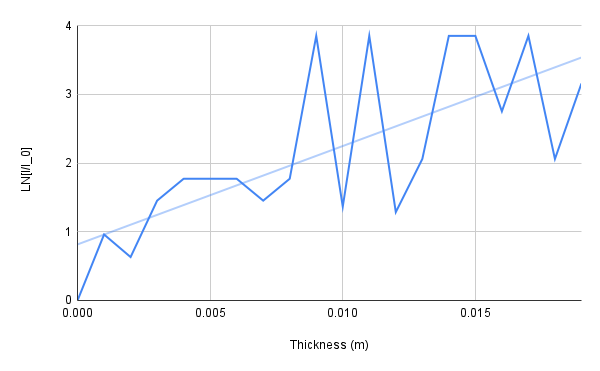
\includegraphics[width=\textwidth]{strontium.png}
        \caption{Strontium-90 Count Rate vs. ln(Thickness), $-\ln(I/I_0) = \mu x$ plotted with $\mu \approx (1.4 \pm 0.3) \times 10^2$}
        \label{fig:cesium}
    \end{minipage}
    \hfill
    \begin{minipage}{0.45\textwidth}
        \centering
        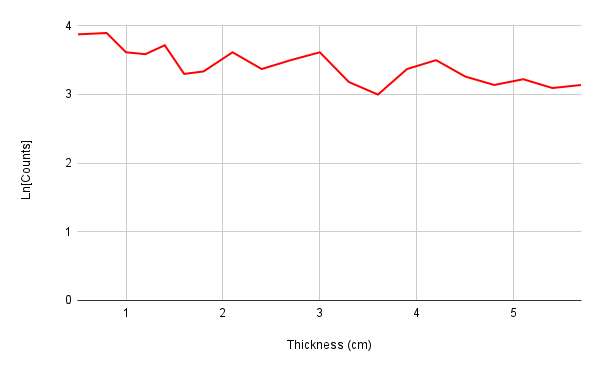
\includegraphics[width=\textwidth]{cesium.png}
        \caption{Cesium-137 Count Rate vs. ln(Thickness), $-\ln(I/I_0) = \mu x$ plotted with $\mu \approx (5 \pm 1) \times 10^1$}
        \label{fig:strontium}
    \end{minipage}
\end{figure}

\section{Thickness}

We see that our strontium reaches approximately $1/e$ or $\approx 36.7$\% of it's original intensity when
the thickness is approximately 0.3 cm, or about 3 cardboard sheets. For our cesium source, we see this value to be
around 2.7 cm, with 8 cardboard and 8 metal sheets.

\section{Banana Equivalent}

If for one year, the dosage is $\text{Activity} \times \text{DCF}$, and 3 hours is 3/8760, then:

\begin{align*}
    D &= A \times DCF \times \frac{3}{8760} \\
    D_{\text{Sr-90}} &= (3700\text{ Bq})(2.8 \times 10^{-8}\text{ Sv/Bq})(3/8760\text{ years}) \approx 3.55 \times 10^{-8} \\
    D_{\text{Cs-137}} &=  (185000\text{ Bq})(1.3 \times 10^{-8}\text{ Sv/Bq})(3/8760\text{ years}) \approx 8.24 \times 10^{-7} \\
    D_{\text{total}} &= D_{\text{Sr-90}} + D_{\text{Cs-137}} = 8.59 \times 10^{-7}\text{ Sv}
\end{align*}

So assuming we swallow them both, we now convert the total to our banana equivalent dosage. The lab manual states that the dosage of eating
a single banana is approximately $0.0000001 = 1 \times 10^{-7}$ Sv. So, a radiation dosage of 
$8.59 \times 10^{-7}$ would be the same as eating around 8.59 bananas, i.e. $BED = 8.59$.

\begin{thebibliography}{9}
    \bibitem{labmanual} 
    Department of Physics. \textit{PHYS 126 Lab Manual}. University of Alberta, 2025.

    \bibitem{person}
    TA assisted with the lab, and provided guidance on the data collection and analysis.

    \bibitem{person}
    Lab partner Morgann Reinhart assisted with the data collection and analysis.
    
\end{thebibliography}

\end{document}
